\section{Design}

In this section, we discuss the design and implementation of our safety guardrails.

\subsection{Background}

We assume agents are fundamentally benign, but might issue unnecessary commands that can be potentially destructive. But enforcing human verification on all operations diminishes the efficiency of AIOps. We want to balance agent autonomy with system safety. However, ensuring agents' reliability in generic use case is difficult, and we want to apply some constraints to make the problem more approachable. We want to study agents' reliability under the context of AIOpsLab, a holistic framework for AI agents evaluation. This framework benchmarks AI agents' accuracy and efficiency. We focus on Kubernetes environment. Mainly, we apply constraints around \textit{kubectl} \cite{Kubernetes_2024}, the command line tool managing Kubernetes clusters. 

\begin{figure}[htbp]
    \centering
    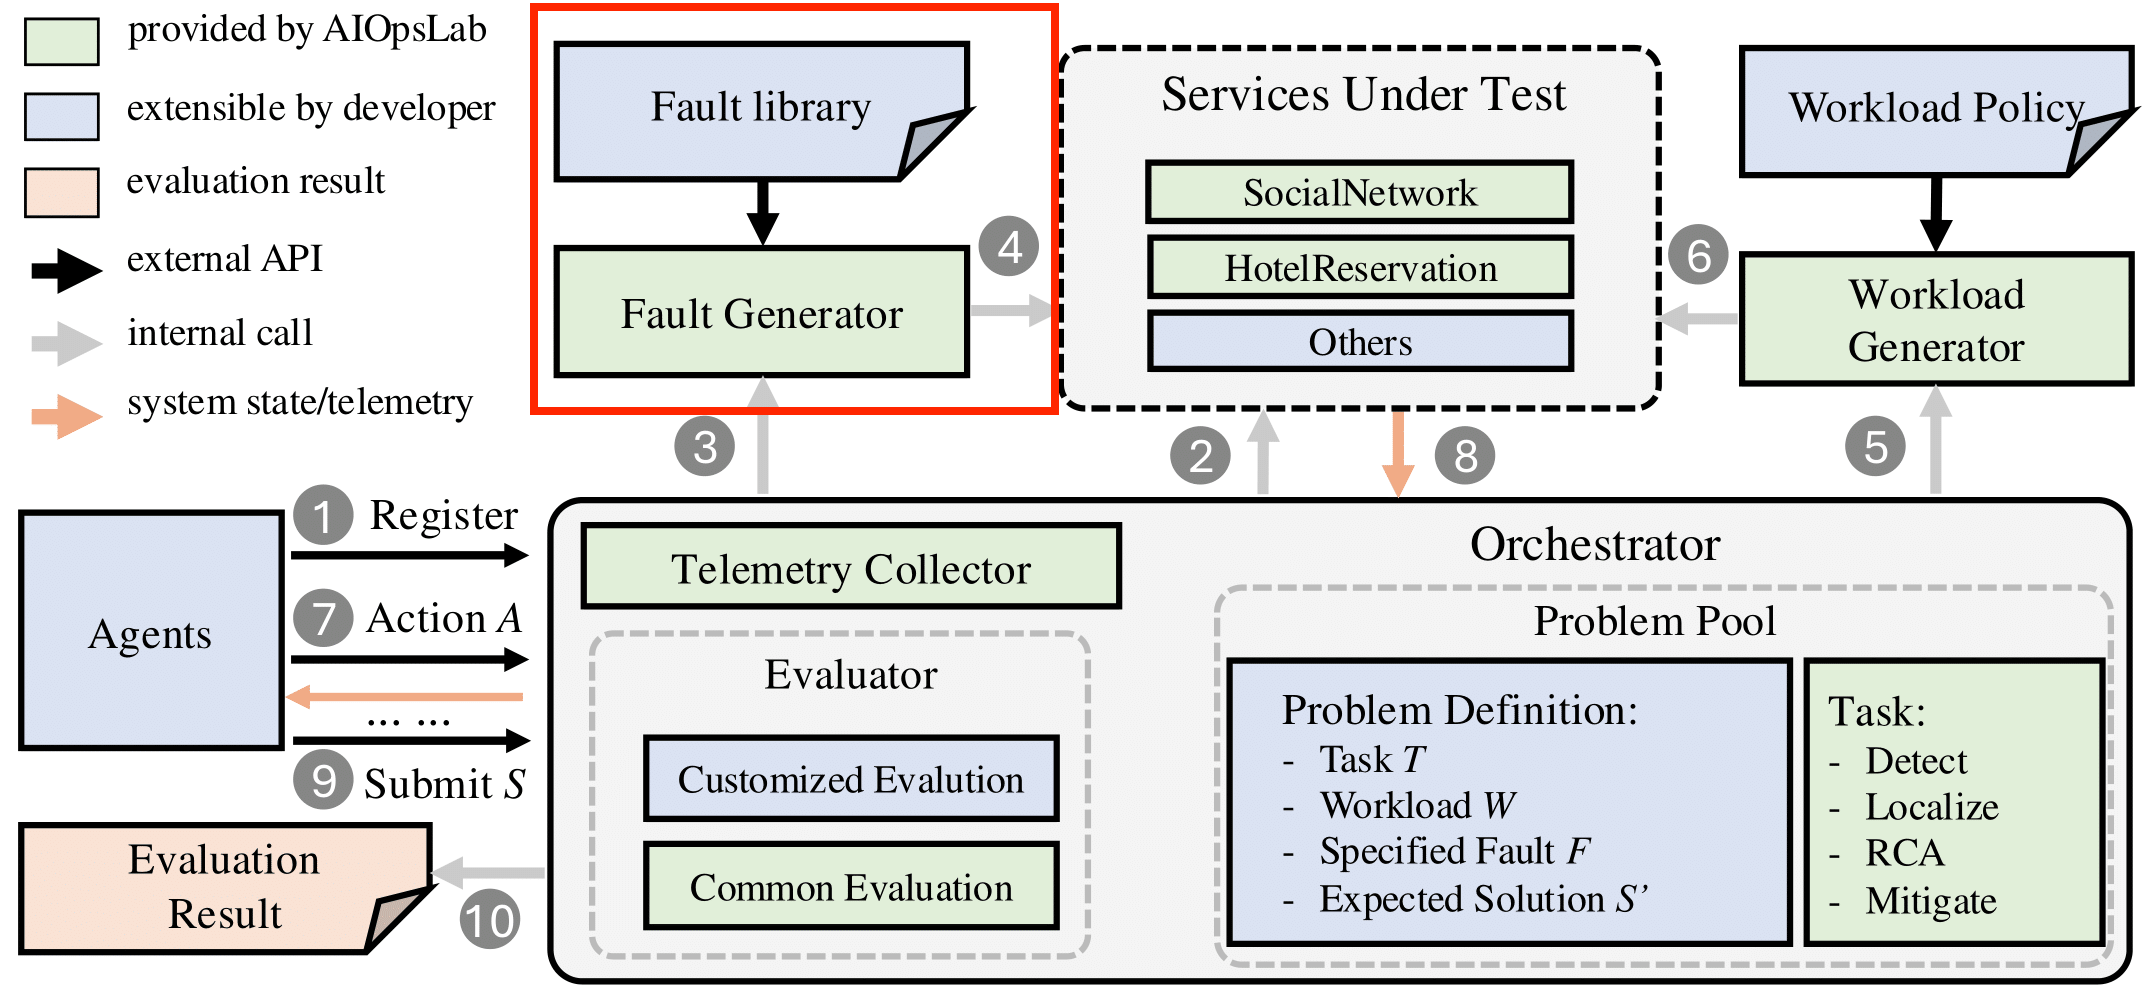
\includegraphics[width=0.5\textwidth]{fig1.png}
    \caption{AIOpsLab infrastructure. Step 4 here demonstrates the procedure on fault injection into the services under test.}
    \label{fig:example}
\end{figure}

\subsection{Intuition}

Agent $A$ applies operation $O$ on resource $R$. Without constraints, this combination yields environment change $E$. However, with both $O$ and $R$ restricted, such that $O_A \subseteq O$, $R_A \subseteq R$, then the potential output space would be limited to $E_A \subseteq E$
\[ O(R) \rightarrow E \]
\[ O_A(R_A) \rightarrow E_A \]

Therefore, we want to enforce agents to operate on mutable resources without the help of restricted commands.

\paragraph{Mutable Resource} AIOpsLab generates determined scenarios, called \textit{Problem}, to ask agents to complete a specific task, e.g. error localization. In the process of generating problem, the framework creates a functioning cluster, and inject faults into designated resource (figure-\ref{fig:example}). For example, the framework intentionally modify a pod's port configuration to simulate pod misconfiguration. Therefore, resources that framework touches upon are potentially faulty, and they are considered mutable.

\paragraph{Restricted Command} Each problem has a known scope, and it corresponds to a list of potential commands to address the issue. Using the port misconfiguration example, deleting or restarting the pod will not resolve the issue, but will bring down the pod for a period of time. These operations damage system's availability for no benefit.



% We want to to balance agent autonomy with system safety by introducing lightweight, context-aware guardrails. The system assumes agents are fundamentally benign, but might issue unnecessary commands that can be potentially destructive. We don’t restrict any read commands, as they don’t pose any risk, and allows the agent to gain contextual information. 

% Furthermore, faults are injected into the system through modifying some elements. Intuitively, since these elements were modified, they naturally should be changed during the fault mitigation process. These elements are considered "mutables", and anything  not in the mutable list should not be changed by the agent. 

\subsection{Implementation}

Existing implementation lacks the observability and traceability of fault injection operations across the system. We changed all fault injection methods to return mutable resources in format of "resource type/resource name", e.g. a pod named \textit{geo-523} is encoded as \textit{pod/geo-523}. This format aligns with kubectl's resource output when we use "-o name" option. This approach has two benefits. First, we can directly use mutable resources' name to compare with kubectl's resource, no additional naming translation required. Second, we add scope to different mutable resources, secure operations from different levels. Exposing mutable resources into the orchestrator allows us to verify agents' operations in runtime.

AIOpsLab provides a function named \textit{exec\_shell} for agents to execute arbitrary bash commands in shell, and agents utilize this handler to interact with the cluster via kubectl. Our goal is to verify agents' kubectl commands beforehand. Inspection commands like \textit{kubectl get} introduce no modification to the system, and we consider them as benign by default. Resource modification commands, e.g. \textit{kubectl apply}, is the input space that we worry about. Luckily, these commands have dry run support for us to learn the impact before the actual modification. The approach is clear now. First, we intercept agents' kubectl commands, and execute them in dry run mode to learn the impact. Second, we compare the returned resource list with our mutable resource list. If the returned resource list is not a subset of our mutable resource list, we forbid the operation. Otherwise, the agent has the freedom to apply its modifications. This pod-level fine-grained validation enables session-level guardrail, preventing unintentional destructive operations.

% In order to enhance the observability and traceability of fault injection operations across the system, we introduced a structured return mechanism across all fault injection methods. Specifically, these methods now return a list of mutable elements that were affected by the fault injection. This change allows the orchestrator to store these modified elements in a session context. 

% In the execution time, the session's mutable objects are passed to shell for execution. Before executing the command passed by the agent, a command validation function first dry runs the command to see the resource it targets, and checks whether that resource is in the mutable list. If the command attempts to modify an element that's not in the mutable list, the system blocks it with "permission denied" error. This verification enables session-level guardrails to enforce context-aware resource validation. 

Furthermore, we strengthened the guardrail by introducing a forbidden pattern filter, which explicitly blocks high-risk commands depending on the context of the fault injected. For example, a port misconfiguration problem doesn't need commands like delete pod or rollout restart to resolve the issue. These types of destructive or cluster-level operations go beyond the intended scope of the fault and can introduce unnecessary disruption. By explicitly blocking such commands through forbidden pattern checks, the system ensures that agents and users operate strictly within the context of the injected fault and only modify the relevant mutable resources, preserving system stability while enabling targeted mitigation.
